\section{Introduction}

\lettrine[findent=2pt]{\textbf{A}}{} cidade do Rio de Janeiro, localizada no
estado do Rio de Janeiro, no Brasil, é uma das 50 cidades mais lindas do
mundo, segundo sites de viagem como Conde Nast Traveler \cite{travelRio}, além
de ser senso comum entre as brasileiras e os brasileiros. Isso traz muita
visibilidade para a capital e com isso, os turistas. Apesar disso, existem
regiões menos visitadas pela população em geral, dentre essas, está Bangu, um
bairro localizado na zona oeste do Rio. É um dos distritos mais populosos do
Rio de Janeiro, com mais de 200 mil habitantes, segundo o Armazenzinho do Rio
de Janeiro \cite{banguSecretaria}. A região de Bangu é uma das mais
quentes da cidade, com as maiores temperaturas máximas da cidade, em média,
(nas estações registradas), segundo o Instituto Nacional de Metereologia
(INMET) \cite{inmetBangu}. 

Nessa região, o quimíco ozônio apresenta concentração muito alta e é
considerada, algumas vezes, inadequada pelos índices de qualidade do ar. Na
maioria dos anos, o índice foi maior do que todas as outras estações, segundo
os dados de monitoramento da qualidade do ar do Data.Rio, da prefeitura da
cidade \cite{datasetAir}, como apresentado na Figura \ref{fig:graph1}.
Exploraremos esses dados ao longo do texto. O motivo de ter capturado as
máximas, ao invés das mínimas ou médias é a importância que elas no caso de
dados faltantes, já que quando se faz a média, ao não ter a medição em
determinado período com relativas baixas da quantidade, a média torna-se mais
alta do que realmente é, e vice-versa. 

\begin{figure}
    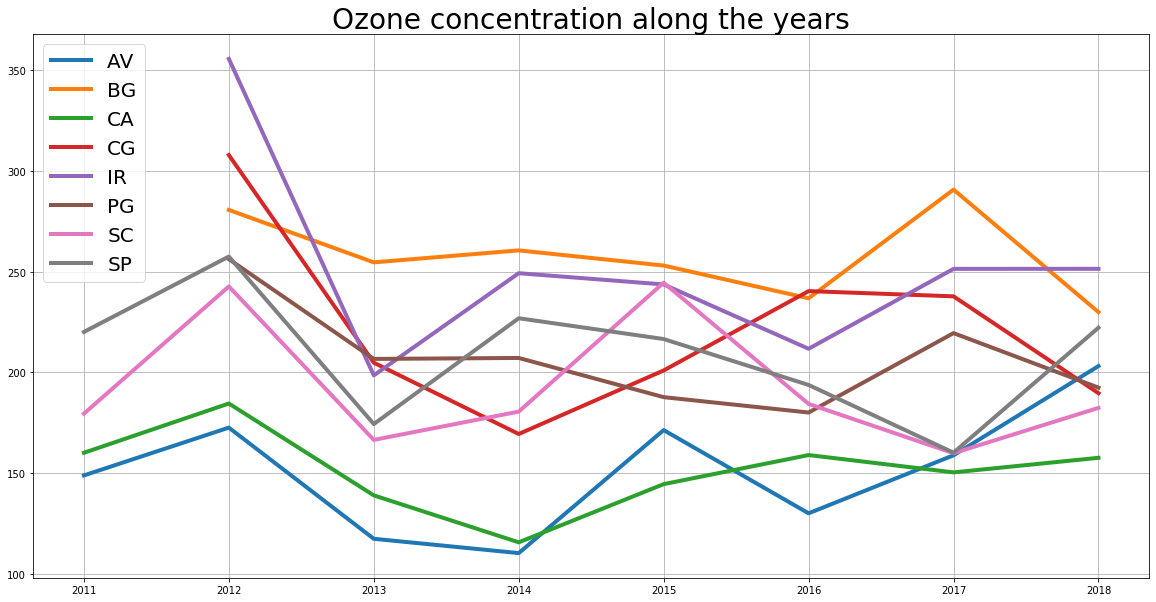
\includegraphics[width=\linewidth]{img/graphic1.png}
    \caption{Um gráfico com as máximas do gás ozônio entre os anos de 2012 a
    2018 nas 8 estações registradas. Bangu é representada pela linha laranja
    (BG).}
    \label{fig:graph1}
\end{figure}

Mas também pensando nisso, utilizando o mesmo banco de dados, é possível ver
que a quantidade média de gás ozônio em todo o período de estudo (2012 -
2018), é maior na região de Bangu, como é possível ver na Figura
\ref{fig:graph2}. Outra região que também assusta com sua média é Pedra de
Guaratiba, porém, vamos nos atentar ao bairro de Bangu. 

\begin{figure}
    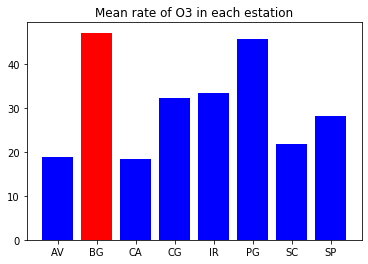
\includegraphics[width=\linewidth]{img/graphic2.png}
    \caption{Gráfico com a média de gás ozônio no período de 2012 a 2018.
    Bangu está sinalizado em vermelho e apresenta a maior das médias. Os
    rótulos são: \{AV: Copacabana, BG: Bangu, CA: Centro, CG: Campo Grande,
    IR: Irajá, PG: Pedra da Guaratiba, SC: São Cristóvão, SP: Tijuca\}}
    \label{fig:graph2}
\end{figure}

A partir dessas visualizações, surge grande interesse no entendimento do
ozônio nessa região, para posterior análise do impacto causado. 

Neste trabalho, dividirei minhas atenções entre o estudo de séries temporais,
em particular sobre a concentração de ozônio ao longo dos anos de 2012 a 2018
e análise de alguns métodos na literatura de previsão. Esses estudos pretendem
seguir o livro Forecasting, de Rob Hyndman and George Athanasopoulos
\cite{forecasting}. No outro sentido, este livro pretende realizar uma crítica
à qualidade do ar naquela região e introduzir possíveis análises das
consequências, lançando mão de inferência causal para potenciais futuros
trabalhos. 

Diferente da análise de amostras aleatórias de observações, discutidas em
outros contextos estatísticos, a série temporal é baseada em valores
sucessivos que representam medidas tomadas em intervalos de espaço igualmente
espaçados. Isto é, trata-se de uma observação ao longo do tempo. A
concentração de ozônio vai de encontro com essa definição, pois sua medida é
captada a cada hora. A partir desses dados, podemos inferir algumas análises. 

O banco de dados é conduzido pelo MonitorAr-Rio, que conta com oito estações
espalhadas pela cidade e uma unidade móvel.  Esse órgão emite um Boletim
Diário, onde descreve condições metereológicas das últimas 24 horas e da
qualidade do ar. Também propõe uma tendência para o próximo dia. Mais
informações sobre esse boletim podem ser encontradas em \cite{boletim}. Para
esse trabalho, coletei os dados sobre informações horárias de diversos
índices, dentre eles Temperatura, Velocidade do Vento e Concentração de vários
poluentes. São essas informações que me interessam. Na imagem \ref{boletim} é
mostrado um boletim do dia 6 de novembro de 2019. Nesse dia, Bangu registrou
um nível de ozônio tão alto que a qualidade do ar foi considerada como má. São
com essas premissas que inicio meu trabalho. 

\begin{figure*}[!ht]  
    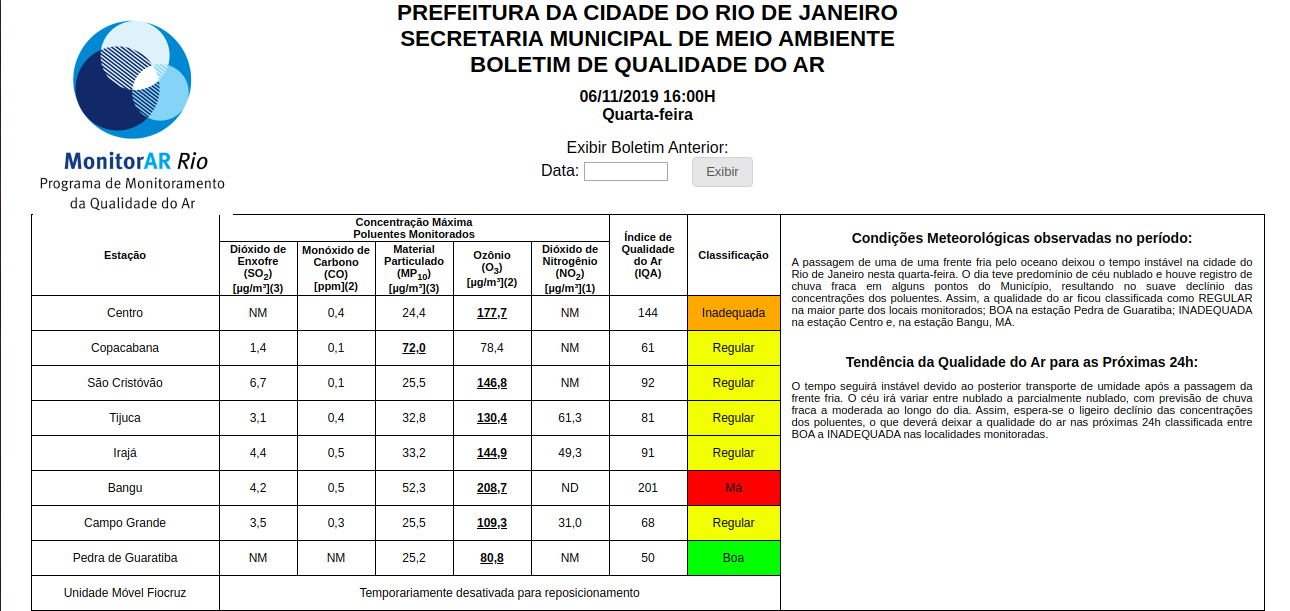
\includegraphics[width=\linewidth]{img/boletim6-11-2019.png}
    \caption{Boletim registrado no dia 06/11/2019}
    \label{boletim}
\end{figure*}

\section{Metodologia}

Este trabalho busca um referencial bibliográfico a fim de compreender o
conhecimento adquirido na área de séries temporais, através de livros e
artigos devidamente citados. 

As análises numéricas foram realizadas na linguagem Python através da
plataforma do Jupyter Notebook, devido à fácil visualização dos gráficos.
Esses gráficos que foram gerados pelas Bibliotecas \textit{Pandas} e
\textit{Matplotlib.pyplot}. Veja Apêndice D.

O banco de dados é disponibilizado pelo Data.Rio em formato \textit{CSV} e
apresenta os dados numéricos. Entretanto, ele apresenta muitos dados
faltantes, devido a manutenções realizadas nas estações. O tratamento para a
maioria dos cálculos aqui apresentados desconsidera-os, porém, para futuros
trabalhos, pretende-se estimar esses valores. 